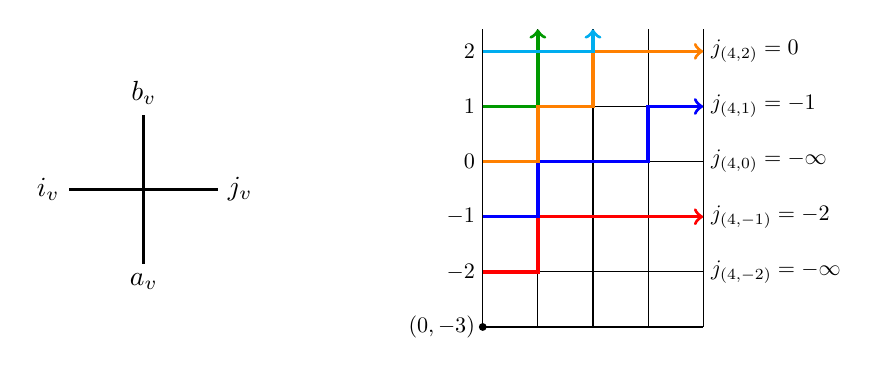
\begin{tikzpicture}[scale=0.7]

  %--- Left subfigure: labels around a vertex v
  \begin{scope}[shift={(-7.5,1.5)}, scale=0.9]
    \draw[line width=1pt] (0,0) -- ++(3,0);
    \draw[line width=1pt] (1.5,-1.5) -- ++(0,3);

    \node[anchor=east]  at (0,0)   {$i_v$};
    \node[anchor=west]  at (3,0)   {$j_v$};
    \node[anchor=north] at (1.5,-1.5) {$a_v$};
    \node[anchor=south] at (1.5,1.5)  {$b_v$};
  \end{scope}

  %--- Right subfigure: grid and colored arrows
  \draw (0,-1) grid (4,4.4);

  % colored paths (only terminal segment carries the arrowhead)
  \draw[red,   very thick, ->] (0,0) -- ++(1,0) -- ++(0,1) -- ++(3,0);
  \draw[blue,  very thick, ->] (0,1) -- ++(1,0) -- ++(0,1) -- ++(2,0) -- ++(0,1) -- ++(1,0);
  \draw[green!60!black, very thick, ->] (0,3) -- ++(1,0) -- ++(0,1.4);
  \draw[orange,very thick, ->] (0,2) -- ++(1,0) -- ++(0,1) -- ++(1,0) -- ++(0,1) -- ++(2,0);
  \draw[cyan,  very thick, ->] (0,4) -- ++(2,0) -- ++(0,0.4);

  % left boundary labels (colors of incoming arrows); y = -2,...,2
  \foreach \y in {-2,...,2} {
    \node[anchor=east, scale=0.8] at (0,\y+2) {$\y$};
  }

  % marked point and its label
  \node[circle, fill, inner sep=1pt] at (0,-1) {};
  \node[anchor=east, scale=0.8] at (0,-1) {$(0,-3)$};

  % right boundary j-values
  \node[anchor=west, scale=0.8] at (4,0) {$j_{(4,-2)}=-\infty$};
  \node[anchor=west, scale=0.8] at (4,1) {$j_{(4,-1)}=-2$};
  \node[anchor=west, scale=0.8] at (4,2) {$j_{(4,0)}=-\infty$};
  \node[anchor=west, scale=0.8] at (4,3) {$j_{(4,1)}=-1$};
  \node[anchor=west, scale=0.8] at (4,4) {$j_{(4,2)}=0$};

\end{tikzpicture}